\documentclass[10pt]{article}
\usepackage[includeheadfoot,letterpaper,centering,margin=0.75in]{geometry}

\usepackage{graphicx}
\usepackage{epstopdf}
\usepackage{amsmath}
\usepackage{amssymb}
\usepackage{hyperref}
\usepackage{fancyhdr}
\usepackage{lastpage}
\usepackage{float}
\usepackage{booktabs}


% -------------------------------------------------------------------
% Styling for the listings package for python
% -------------------------------------------------------------------
\usepackage[T1]{fontenc}
\usepackage[scaled]{beramono}
\usepackage{listings}
\usepackage{upquote}
\usepackage[usenames]{color}
\usepackage{setspace}

\definecolor{gray}{gray}{0.5}

\lstset{
  language=Python,
  basicstyle=\ttfamily\small\setstretch{1},
  showstringspaces=false,
  alsoletter={1234567890},
  morekeywords={models, lambda, forms},
  otherkeywords={\ , \}, \{},
  emphstyle=\color{black}\bfseries,
  upquote=true,
  morecomment=[s]{"""}{"""},
  commentstyle=\color{gray}\slshape,
  tabsize=4,
  formfeed=\newpage,
  numbers=left, 
  numberstyle=\tiny, 
  stepnumber=1, 
  numbersep=5pt,
  frame=lines
}

% -------------------------------------------------------------------
% Include code with a title
% -------------------------------------------------------------------
\newcommand{\code}[2]{
  \subsection*{#1}
  \lstinputlisting{#2}
}

% -------------------------------------------------------------------
% Student and Assignment Specifics
% -------------------------------------------------------------------
\newcommand{\assignclass}{CocoNuTs - MATH 303}

\newcommand{\assignstudent}{Michael Arnold}

\begin{document}

\begin{figure}[h]
\begin{center}
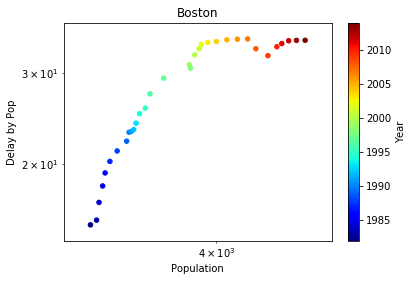
\includegraphics[scale=.6]{1.png}
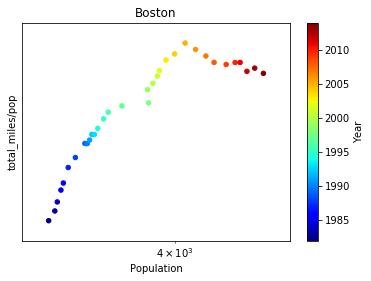
\includegraphics[scale=.6]{2.png}
\end{center}
\end{figure}
\pagebreak
\begin{figure}[h]
\begin{center}
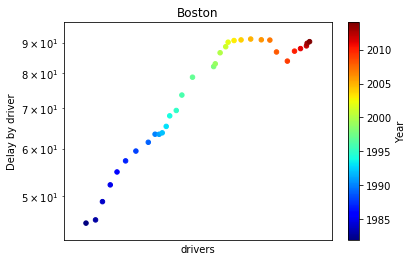
\includegraphics[scale=.6]{3.png}
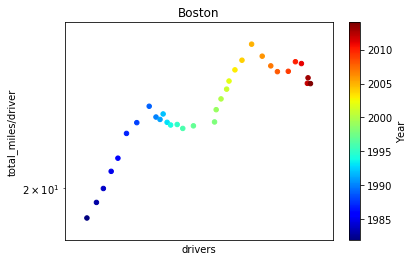
\includegraphics[scale=.6]{4.png}
\end{center}
\end{figure}
\end{document}

